\documentclass[11pt]{sdm_internship}

\usepackage{graphicx}
\graphicspath{{../img/}}

\usepackage{subcaption}
\usepackage{cleveref}
\usepackage{comment}
\pagestyle{plain}

\usepackage{hyperref}
\usepackage{url} \urlstyle{sf}
\newcommand{\email}[1]{\href{mailto:#1}{#1}}

\usepackage{xspace}

\usepackage[dvipsnames]{xcolor}
\newcommand{\addref}[1]{\colorbox{TealBlue!100}{\textcolor{white}{\textbf{$[$\ifx&#1&\ \else#1\fi$]$}}}}
\newcommand{\todo}[1]{\colorbox{Red!75}{\textcolor{white}{\textbf{TODO\ifx&#1&\else: #1\fi}}}}
\newcommand{\done}{\colorbox{YellowGreen!100}{\textcolor{white}{\textbf{DONE}}}}
\newcommand{\review}{\colorbox{YellowOrange!100}{\textcolor{white}{\textbf{REVIEW}}}}

\newcommand{\dspot}{DSpot\xspace}

\usepackage{minted}

\usepackage{ragged2e}

\title{Adapting Amplified Unit Tests for Human Comprehension}

\author{Simon \textsc{Bihel}}
\supervisorOne{Benoit \textsc{Baudry}}
\supervisorTwo{~}
\team{KTH Royal Institute of Technology}
\school{ens-Rennes}

\domain{Domain: Software Engineering --- Artificial Intelligence}

\abstract{%
  \justify{%
    \todo{}
  }
}


% Ought to be between 30 and 50 pages

\begin{document}
\maketitle

% ================================================================================
\section*{Introduction}%
\label{sec:intro}%
\addcontentsline{toc}{section}{\nameref{sec:intro}}
\todo{}


% ================================================================================
\section{Background}%
\label{sec:background}
\todo{intro}

% --------------------------------------------------------------------------------
\subsection{Software Testing}%
\label{ssec:software_testing}
\todo{Why are we testing software and how do we do it}

% --------------------------------------------------------------------------------
\subsection{Elementary Metrics}%
\label{ssec:elementary_metrics}
\todo{What are the basic metrics}

\todo{What are their limits}

% --------------------------------------------------------------------------------
\subsection{Mutation Testing}%
\label{ssec:mutation_testing}
\begin{figure}
  \centering
  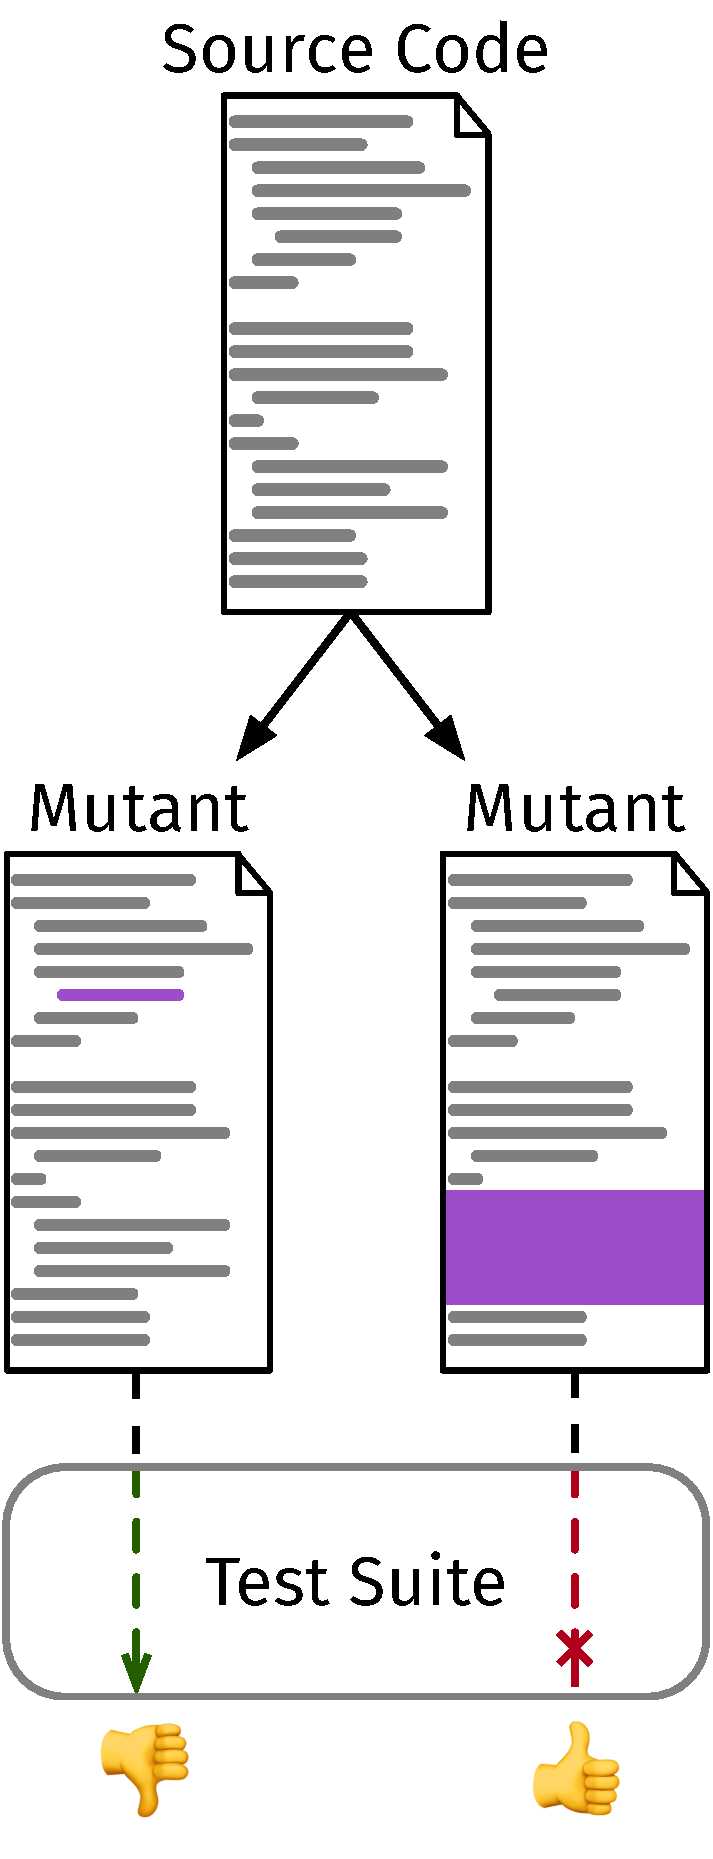
\includegraphics[width=9em]{mutation_testing}
  \caption{}%
\label{fig:spaces}
\end{figure}
% Introduction
Mutation testing is a method used to assess the quality of a test suite, grading it with a metric called \textit{mutation score}.
The idea is to insert bugs in the software and see if these faulty versions still pass the tests or not.
We call the derived versions \textit{mutants}, hence the name mutation testing.
The global process is depicted in~\figurename~\ref{fig:spaces}.
\todo{enrich}
\addref{fundational papers}

% Mutators
\todo{examples of mutators}

% Difficulties
\todo{why is it not widespread in the industry}
\begin{itemize}
  \item slow
  \item not understood (difficult to know what the improvements to the tests should be)
  \item useless mutants
\end{itemize}
\cite{jia2011analysis}

% Pitest
PIT\footnote{\url{http://pitest.org/}}~\cite{coles2016pit} is a mutation testing tool for Java.

\todo{what is great about it}

\todo{it is deterministic}

% --------------------------------------------------------------------------------
\subsection{Software Diversification}%
\label{ssec:software_diversification}
\todo{}

% --------------------------------------------------------------------------------
\subsection{The Need for Easy-to-use Tools}%
\label{ssec:software_testing}
\todo{easy to understand}
\todo{useful for surveys}


% ================================================================================
\section{Test Suite Amplification}%
\label{sec:test_suite_amplification}
\todo{intro}

% --------------------------------------------------------------------------------
\subsection{Related Works}%
\label{ssec:dspot_related_works}
\todo{}

% --------------------------------------------------------------------------------
\subsection{\dspot{}}%
\label{ssec:dspot}
\begin{figure}
  \centering
  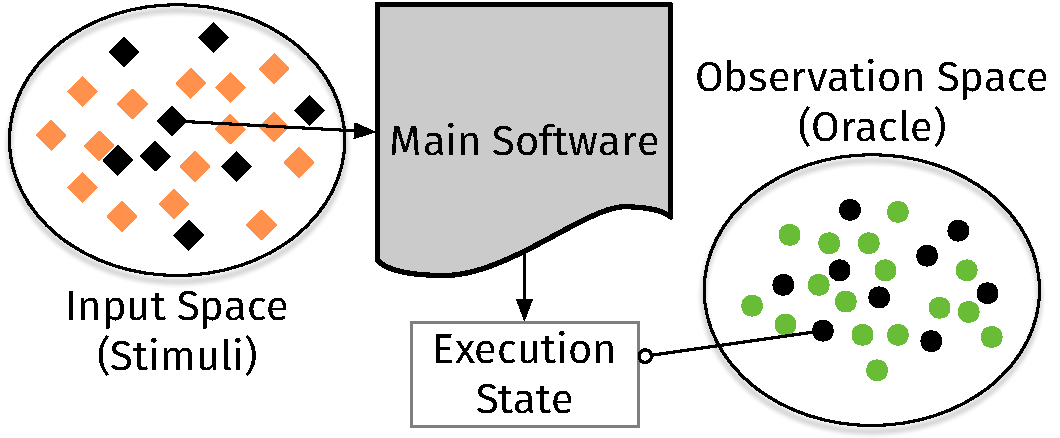
\includegraphics[width=22em]{spaces}
  \caption{On the left, the testing input space is composed by specified input points (orange diamonds) and unspecified input points (black diamonds). On the right, the observation space over a given program state depicts the assertions of tests. The green circles are values that are already asserted in the existing test suite, the newly added assertions are shown as black circles.}%
\label{fig:spaces}
\end{figure}
\todo{}
\footnote{\url{https://github.com/STAMP-project/dspot}}\addref{dspot papers}


% ================================================================================
\section{Problem Statement}%
\label{sec:problem_statement}

% --------------------------------------------------------------------------------
\subsection{The Need for Unit Test Cases Documentation}%
\label{ssec:need_doc}
\todo{}
\cite{li2016automatically}

% --------------------------------------------------------------------------------
\subsection{The Generated Random Noise}%
\label{ssec:random_noise}
\todo{}

\todo{lack of why information}


% ================================================================================
\section{Related Works}%
\label{sec:related_works}
\todo{}

% --------------------------------------------------------------------------------
\subsection{Automatic Test Case Documentation}%
\label{ssec:test_doc}
\todo{}

% --------------------------------------------------------------------------------
\subsection{Source Code Change Documentation}%
\label{ssec:commit_generation}
\todo{}


% ================================================================================
\section{Contribution}%
\label{sec:contribution}
\todo{}

% --------------------------------------------------------------------------------
\subsection{Identifying Amplifications}%
\label{ssec:retrieve_amplifications}
\todo{}

% --------------------------------------------------------------------------------
\subsection{Minimisation}%
\label{ssec:minimisation}
\todo{}
\todo{put slicing before?}

% --------------------------------------------------------------------------------
\subsection{Replace or Keep}%
\label{ssec:replace_keep}
\todo{}

% --------------------------------------------------------------------------------
\subsection{Focus}%
\label{ssec:focus}
\todo{}

% --------------------------------------------------------------------------------
\subsection{Slicing}%
\label{ssec:slicing}
\todo{}

% --------------------------------------------------------------------------------
\subsection{Natural Language Description}%
\label{ssec:nl_description}
\todo{}

% --------------------------------------------------------------------------------
\subsection{Ranking}%
\label{ssec:ranking}
\todo{}


% ================================================================================
\section{Evaluation}%
\label{sec:eval}
\todo{}


% ================================================================================
\section*{Conclusion}%
\label{sec:conclu}%
\addcontentsline{toc}{section}{\nameref{sec:conclu}}
\todo{}


% ================================================================================
\section*{Acknowledgments}%
\label{sec:ack}%
\addcontentsline{toc}{section}{\nameref{sec:ack}}
Thanks to Benoit Baudry and Martin Monperrus for their guidance.
Thanks to Benjamin Danglot for his collaboration and all his work on \dspot.
Thanks to Zimin Chen, Nicolas Harrand, He Ye and Long Zhang for making daily life enjoyable.
This internship was supported by the Fondation Rennes 1 and its patrons.
Many thanks to KTH for hosting me.


% ================================================================================
\bibliographystyle{ieeetr}%
\bibliography{../bibl}%
\label{sec:ref}%
\addcontentsline{toc}{section}{\nameref{sec:ref}}

\end{document}
